\textbf{Problem 2: Nyström method and the Fredholm alternative.}

For this problem, the boundary is the unit circle (all points $x,y$ such that $x^2+y^2=1$).  The boundary condition on the circle is of Neumann type, specifically, the normal derivative of the potential (with the normal pointing out of the circle) is
\begin{align}
    \left. \frac{\partial{u}}{\partial{n}} \right|_\Gamma = \frac{1}{3+2\cos\theta +\cos2\theta}
\end{align}

For the interior, the monopole integral formulation of the Neumann problem in 2-D Laplace:
\begin{align}
    \frac{\partial{u}_\Gamma (\vec{x})}{\partial{n}_{\vec{x}}}
    = +\pi\sigma(\vec{x}) - \int_\Gamma^{PV}
    \frac{(\vec{x}-\vec{x}')^Tn_{\vec{x}}}{\norm{\vec{x}-\vec{x}'}^2}\cdot \sigma(\vec{x}') \dd{\Gamma'},
    \qquad \vec{x}\in\Gamma
\end{align}

\begin{enumerate}[label=(\alph*),leftmargin=*,itemsep=0mm]
    
    \item We see that Eqn. (19) is the same as Eqn. (4), except that the 1st term is $+\pi\sigma(\vec{x})$ instead of $-\pi\sigma(\vec{x})$.  Therefore, all else being the same we therefore have that Eqn. (11) is transformed into:
    \begin{align}
        \vec{A} = \begin{pmatrix} \pi - \frac{\pi}{n} & \dots & -\frac{\pi}{n} \\
        \vdots & \ddots & \vdots \\
        -\frac{\pi}{n} & \dots & \pi -\frac{\pi}{n} \end{pmatrix}
        = \pi I - \frac{\pi}{n} J_n
    \end{align}
    
    The rank of matrix $\vec{A}$ is lower than its size and therefore the system of linear-equations is underdetermined, meaning that we cannot find a unique solution to the system, and therefore the interior Neumann problem with either of the boundary conditions has an infinite possible number of solutions.
    
    \item We consider the following boundary condition for the interior Neumann problem on the unit circle:
    \begin{align}
        \left. \frac{\partial{u}}{\partial{n}} \right|_\Gamma
        = \frac{\partial}{\partial{n}}
        \left( \log \sqrt{x^2 + \left( y + 2 \right)^2}
        - \log \sqrt{x^2 + \left( y - 2 \right)^2} \right)
    \end{align}
    
    So, we have that the potential is given by
    \begin{align}
        u(x,y) = \log \sqrt{x^2 + \left( y + 2 \right)^2}
        - \log \sqrt{x^2 + \left( y - 2 \right)^2}
    \end{align}
    
    And the normal derivative of the gradient is
    \begin{align}
        \left. \frac{\partial{u}}{\partial{n}} \right|_\Gamma
        &= \left( \frac{x}{x^2+(y+2)^2} - \frac{x}{x^2+(y-2)^2} \right) \cdot \frac{x}{\sqrt{x^2+y^2}} \nonumber \\
        &\quad + \left( \frac{y+2}{x^2+(y+2)^2} - \frac{y-2}{x^2+(y-2)^2} \right) \cdot \frac{y}{\sqrt{x^2+y^2}}
    \end{align}
    
    Again, because the matrix $\vec{A}$ is of a lower-rank in size, and therefore the system of linear equations is underdetermined such that there are an infinite number of solutions to this problem.  We therefore modify the Nyström method by setting $u$ at a point $\vec{x}_0$, such that an additional constraint is provided to this problem, and use this extra constrain to ensure that the matrix $\vec{A}$ is full-rank.
    
    Let us say that $\vec{x}_0 = (0,0)$ such that the analytic potential $u_{\vec{x}_0} = 0$.  We substitute this into the last row of the matrix by considering the discrete form
    \begin{align}
        u(\vec{x}_0) = \sum_{j=1}^n - \frac{2\pi}{n} \ln \norm{\vec{x}_0-\vec{x}_j} \sigma_{nj}
    \end{align}
    
    We then use our answer from Q1(c) and compare the difference between the exact analytical solution and its numerical approximation.  For $n=5,20,50$, we plot the exterior fields outside the unit circle and compare the analytical solution with its numerical approximation (Fig. \ref{prj3_qn2b_field})

    \begin{figure*}[h!]
    \centering
    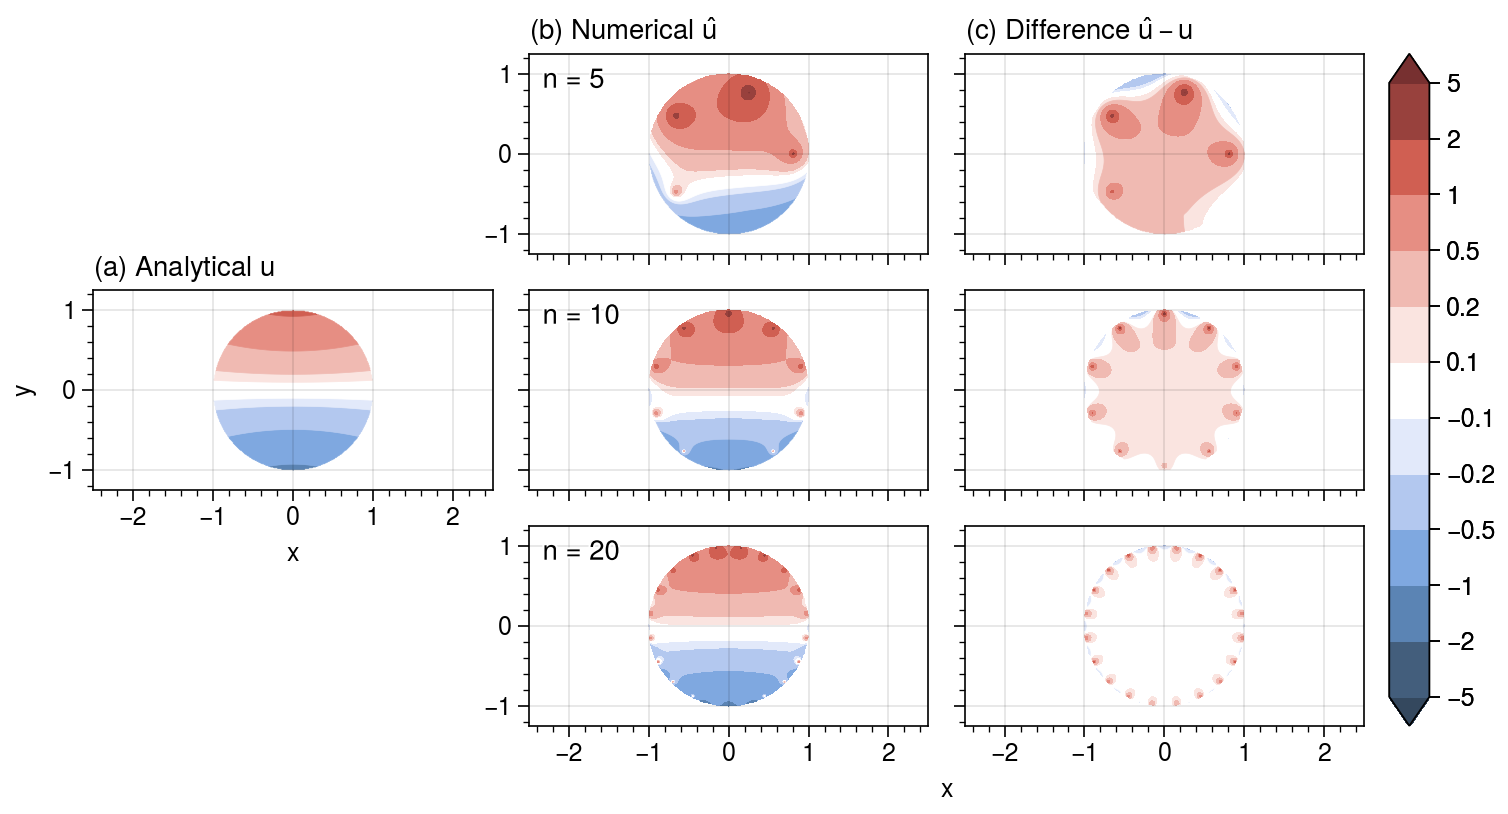
\includegraphics[width=\textwidth]{figures/prj3_qn2b_field.png}\\
    \caption{}
    \label{prj3_qn2b_field}
    \end{figure*}
    
    For test circles with radii (i) $1-\frac{1}{4}$, (ii) $1-\frac{1}{16}$ and (iii) $1-\frac{1}{256}$, we plot the errors for $n$ test points against $n$ in Fig. \ref{prj3_qn1dqn2b}b.  We see that the convergence rate for (i) and (ii) are largely of 1st-order convergence.  However, (iii) order of convergence is non algebraic until around $n=1500$ where the order of convergence then transitions to 2nd order.
    
    
\end{enumerate}